\documentclass{mwart}
\usepackage[utf8]{inputenc}
\usepackage{polski}
\usepackage{lmodern,microtype}
\usepackage{tikz}
\usetikzlibrary{trees}
\usetikzlibrary{shadows}
\usepackage[hidelinks, breaklinks, pdfusetitle, pdfdisplaydoctitle]{hyperref}
\usepackage{float}
% Autorzy i metadane
\author{Michał Anczykowski\and Daria Grzelak\and Jan Ratajczyk}
\title{Projekt zespołowy --- opracowanie zadania z prawdopodobieństwa}
\date{\today}
% Początek dokumentu
\begin{document}
\maketitle
Celem niniejszego projektu jest opracowanie jednego ze starych zadań z matury rozszerzonej z~matematyki. Jest to zadanie 11 z~matury z~2~czerwca~2023~roku w~formule 2015, a~jego treść jest następująca:

\begin{quote}
W pudełku umieszczono $n$~kul ($n \geq 3$), wśród których dokładnie 2~kule są czarne, a~pozostałe kule są białe. Z~tego~pudełka losujemy jedną kulę i~odkładamy ją na bok. Jeżeli wylosowana kula jest biała, to do~pudełka wrzucamy kulę czarną, a~gdy wylosowana kula jest czarna, to do~pudełka wrzucamy kulę białą. Po przeprowadzonej w~ten~sposób zmianie zawartości prawdopodobieństwo wylosowania kuli białej z~tego~pudełka jest równe $\frac{37}{50}$. Oblicz $n$\footnote{Pełen arkusz można znaleźć na stronie \href{https://arkusze.pl/maturalne/matematyka-2023-czerwiec-matura-stara-rozszerzona.pdf}{Arkusze.pl}.}.
\end{quote}

Dalej trzeba przedstawić rozwiązanie, a także je uogólnić --- największą trudność sprawia fakt, że prawdopodobieństwa nie można sobie wpisać losowo, chyba że zrobimy to tak, że prawdopodobieństwo można wpisać dowolne, ale jeśli nie będzie wychodziła liczba naturalna jako n, to będzie wyświetlać komunikat, że dla takiego prawdopodobieństwa jest brak rozwiązań.

Drzewko (nie jest sparametryzowane, ale już jest wystylizowane):

\begin{figure}[h]
	\centering
	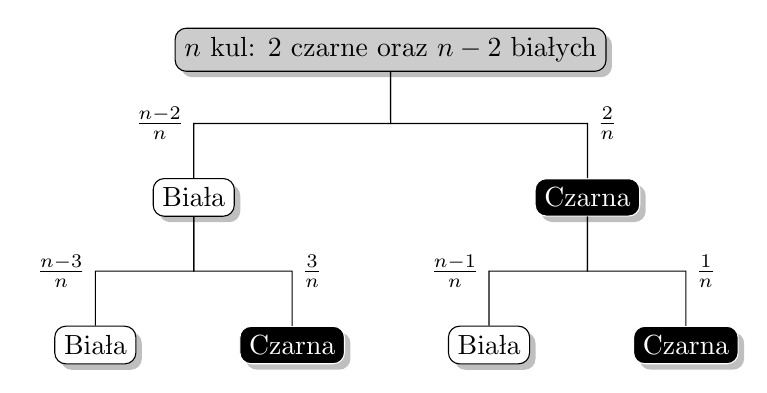
\begin{tikzpicture}[scale=1.25, edge from parent fork down]
		\node [rounded corners, drop shadow, fill=gray!40, draw]{$n$ kul: 2 czarne oraz $n - 2$ białych} [sibling distance=4cm]
			child {node [rounded corners, drop shadow, draw, fill=white] {Biała} [sibling distance = 2cm]
			child {node [rounded corners, drop shadow, draw, fill=white] {Biała}
			edge from parent node [left] {$\frac{n-3}{n}$}
			}
			child {node [rounded corners, drop shadow, draw=white, fill=black] {\textcolor{white}{Czarna}}
			edge from parent node [right] {$\frac{3}{n}$}
			}
			edge from parent node [left] {$\frac{n-2}{n}$}
			}
			child {node [rounded corners, drop shadow, draw=white, fill=black] {\textcolor{white}{Czarna}} [sibling distance = 2cm]
			child {node [rounded corners, drop shadow, draw, fill=white] {Biała}
			edge from parent node [left] {$\frac{n-1}{n}$}
			}
			child {node [rounded corners, drop shadow, draw=white, fill=black] {\textcolor{white}{Czarna}}
			edge from parent node [right] {$\frac{1}{n}$}
			}
			edge from parent node [right] {$\frac{2}{n}$}
			};
	\end{tikzpicture}
\end{figure}
...
\end{document}